% This is samplepaper.tex, a sample chapter demonstrating the
% LLNCS macro package for Springer Computer Science proceedings;
% Version 2.20 of 2017/10/04
%
\documentclass[runningheads]{llncs}
\usepackage[hyphens]{url}
\usepackage{graphicx}
\usepackage{xcolor,colortbl}
\usepackage{mdframed}
\usepackage{multirow}
\usepackage{multicol}
\usepackage{comment}
\usepackage{amsmath}
\usepackage[utf8]{inputenc}
\usepackage[T1]{fontenc}
\usepackage[inline]{enumitem}
% Used for displaying a sample figure. If possible, figure files should
% be included in EPS format.
%
% If you use the hyperref package, please uncomment the following line
% to display URLs in blue roman font according to Springer's eBook style:

\mdfdefinestyle{RQFrame}{
 outerlinewidth=0pt,
 skipabove=0pt,
 skipbelow=0pt,
 innertopmargin=6pt,
 innerbottommargin=0pt,
 linewidth=0pt,
 topline=false,
 rightline=false,
 leftline=false,
 innerrightmargin=4pt,
 innerleftmargin=4pt}

\newcounter{RQCounter}
\newcommand{\RQ}[2]{
\refstepcounter{RQCounter} \label{#1}
\begin{mdframed}[style=RQFrame]\noindent
    \textbf{RQ}$_{\arabic{RQCounter}}$.~\emph{#2}
\end{mdframed}
}
\newcommand{\hr}[1]{\textbf{RQ}$_{\ref{#1}}$}
\definecolor{Gray}{gray}{0.9}
\newcommand{\mysubsec}[1]{\smallskip \emph{\textbf{#1.}}}



\usepackage{hyperref}
\renewcommand\UrlFont{\color{blue}\rmfamily}

\begin{document}

%
\title{Developing and evaluating a hackathon approach to foster cybersecurity learning}
%
%\titlerunning{Abbreviated paper title}
% If the paper title is too long for the running head, you can set
% an abbreviated paper title here
%
\titlerunning{Developing and evaluating a hackathon approach to foster cybersecurity learning}

%\author{Abasi-amefon O. Affia \and Alexander Nolte \and Raimundas Matulevi\v{c}ius }
%\institute{Institute of Computer Science, \\ University of Tartu, Tartu, Estonia,\\
%\email{amefon.affia@ut.ee, alexander.nolte@ut.ee, rma@ut.ee}
%}
%
\authorrunning{}
%\authorrunning{Affia et al.}
%
\maketitle              % typeset the header of the contribution
%
\begin{abstract}
Securing information systems and raising awareness about how to use them securely is one of the significant challenges of the coming years. Hackathons appear to be a good approach because it is useful to train, spread awareness, and encourage people to explore the security of information systems. This paper describes the design and evaluation of a hackathon approach that fosters cybersecurity security. 
Evaluating our approach, we found that the participants attain different levels of cybersecurity learning based on the interactions with the introduced interventions.
%with the interventions stimulate learning at different levels, helping participants achieve cybersecurity learning
% findings
\keywords{Hackathons  \and Security \and Learning \and Action Research.}
\end{abstract}
%
%
% Hackathons are increasingly popular across different domains in recent years including the security domain. 

\section{Introduction}
Technological advancements have led to the ubiquitous availability of data and continue to shape digital innovation \cite{davenport2013analytics}. 
Industry experts predict there will be 6 billion internet users by 2022 \cite{cybersecventures2019} and nearly 26 billion connected devices by 2020 \cite{hung2017gartner}. The increase in devices significantly expands the attack surface for cybercriminals, who are continually developing more advanced and scale able tools to access user sensitive data. %Thus, securing these systems and raising awareness about how to securely use them is one of the great challenges of the coming years.
Thus, it is necessary to build secure systems and train users to use these systems securely.
A critical security measure for the success and growth of information systems is the level of knowledge and awareness among those which build or use these systems. %\cite{mahmoud2015internet}. 
 %Already, more than 4.5 billion records were breached in the first half of 2018\footnote{\url{https://www.gemalto.com/press/Pages/Data-Breaches-Compromised-3-3-Billion-Records-in-First-Half-of-2018.aspx} (accessed at 11/03/2020)}. 
%So,
%However, there is widespread ignorance of likely threats and adversaries with end-users or administrators of these information systems. %In contribution to continuous research, development and innovation in IoT security, methods to improve cybersecurity learning as a contribution to already existing methods for IoT innovation is imperative. 
  %Solving these challenges form a part of digital innovation and such innovations are as a result of collaborative processes in (interdisciplinary) teams rather than as the work of individuals\cite{steen2011benefits}.

We propose to utilize the hackathon format as a way to spreading cybersecurity knowledge to the larger population. Hackathons are time-bounded events during which participants from diverse backgrounds form teams and work on projects that are of interest to them \cite{pe2018designing}. They have seen a steep rise in popularity in recent years and have been organized in a variety of domains including corporations \cite{nolte2018you,komssi2015hackathons}, start-ups \cite{nolte2019touched,cobham2017hackathon1}, (higher) education \cite{porras2019code,kienzler2017learning}, civic engagement, \cite{lodato2016issue,henderson2015getting} and have also been proposed as a tool for teaching to educational curricula in general \cite{abdullah2015stimulating,porras2019code,sakhumuzi2017student,nandi2016hackathons} and to train users in using and building IT systems \cite{weiss2015teaching,kharchenko2016university,boopathi2015learning}. Learning has in fact been cited as one of the key motivations for participants to join hackathons \cite{porras2019code,briscoe2014digital,juell2014public}.

While learning can be considered an essential part of every hackathon prior work provides indication that what organizers want participants to learn can be different from what they actually learn or are interested in learning \cite{medina2019does}. It is thus necessarily to purposefully design hackathons to foster cybersecurity learning but it is at the same time unclear which strategies indeed foster the desired learning outcomes. Our study addresses this gap by developing and evaluating a hackathon approach that aims to foster cybersecurity learning in a hackathon. Based on prior work in the hackathon domain we proposed specific intervention to the hackathon approach thus aiming to answer the following two related research questions:

\RQ{RQ1}{How can different interventions at a hackathon influence learning?}
\RQ{RQ2}{How can these interventions be improved?}

To answer these questions, we conducted an action research study of three teams at a cybersecurity hackathon. The methods and processes to stimulate learning were provided as interventions introduced during the hackathon process. We observed all teams and participants during the hackathon at set intervals during its early, mid, and later phases, administered questionnaires and conducted interviews at the end of the hackathon event.

Our results indicate that the participants interactions with the interventions stimulate learning at different levels, helping participants achieve cybersecurity learning (\hr{RQ1}). 
We also evaluate the perceived usefulness of the interventions to the participants (\hr{RQ1}) and as a result, suggest improvements to the interventions (\hr{RQ2}). %, acquired by observing the perceived cybersecurity learning outcome of the interventions within the teams.

\section{Background}
In the following section we will discuss our work in the context of prior work on hackathons in cybersecurity (section \ref{Sec:relatedworks}) before focusing on learning in particular (section \ref{Sec:designaspects}).

\subsection{Related works}\label{Sec:relatedworks}
Hackathons are intense, uninterrupted and \textit{time-bounded} events, typically of 2-5 days, during which people gather together and form \textit{collocated teams}, in attempts to complete a \textit{project} of interest \cite{nolte2018you,komssi2015hackathons}. Hackathons in the security domain have mainly been used to facilitate training and awareness in the cybersecurity community and to train future cybersecurity professionals.

Although studies on security hackathons exist, most reports focus only on describing the hackathon event.
Kharchenko et al. \cite{kharchenko2016university} presented a case study collection of different cybersecurity hackathons carried out to facilitate university-industry cooperation. 
However, they did not report on an evaluation of the design aspects that fostered cybersecurity learning and the learning objectives of the hackathon. Similarly, the paper by Starov et al. \cite{starov2015hacking}, reports on a hackathon where students were provided comprehensive knowledge in a particular course, then participated in an idea generation and prototype development training.
The emphasis of this study was on start-up development and establishing communication between the university and industry. The study did not show any evaluation of learning objectives or design aspects to foster learning. Finally, Foley et al. \cite{foley2018science} discuss findings from a science hackathon for researchers. Here, researchers were able to explain ongoing their ongoing research in cyber-physical systems (CPS) security based on a shared CPS test-bed.
But, the paper does not report on an evaluation of the design aspects that foster awareness and cybersecurity learning.

Our work is thus different from prior studies on cybersecurity learning at hackathons because we aim to develop and evaluate specific interventions and identify means for improving them.

\subsection{Hackathon Design aspects for Learning}\label{Sec:designaspects}
Designing hackathons that foster learning require careful planning to create a learning environment suitable for learning through problem-solving \cite{case2004between}. Participants should be able to gain sufficient knowledge about cybersecurity to explore and contribute to the development of security solutions within the tight time constraints of the hackathon\cite{kollwitz2019hack}.
Here, we discuss design aspects that have been found in literature to foster cybersecurity learning, and used as a basis for interventions discussed in section \ref{Sec:interventions}.

The early part of each hackathon is for teams to generate ideas aligned to the theme of the event. 
Ideas proposed should be real-world problems that and form the basis of the project they will work on during the event \cite{stoyanov2007effect}. \textbf{Idea generation} allows the participants to involve in self-regulated learning from the investigation of the necessary information, and the pursuit of logical inquiry based on knowledge gained \cite{akcay2009problem}. 
It is thus crucial for hackathons to start with an open idea generation phase \cite{bohmer2015open} where teams can express and refine ideas. 


To encourage cybersecurity learning by solving security issues, it is necessary to provide participants with both domain-specific knowledge and domain generic knowledge for analysis of the problem context in idea generation \cite{stoyanov2007effect}.
\textbf{Security talks} at the hackathon provides participants with an understanding of the security domain and properly recognise the need for security within the current advances in information systems. Security taalks also provide the opportunity for participants to learn new skills \cite{horton2018project} relevant to the security solution.

%given the limited time frame of the hackathon \cite{lara2016hackathons}
One of most prevalent forms of participant support during a hackathon are mentors providing on-demand and assigned guidance to teams in need \cite{soltani2014hackathon,byrne2017iot}. \textbf{Mentor feedback} support teams to scope their solutions, provide suggestions about how approach a problem, and help with (technical) problems given the limited time frame of the hackathon \cite{lara2016hackathons}.
Mentorship also allows participants to receive learning-oriented support, especially when mentors perceive their role as that of a traditional (workplace or educational) mentor \cite{nolte2020support}.

Although participation in the hackathon is voluntary, specific incentives can encourage individuals to participate. \textbf{Competition style} design provide incentives to motivate participants to attempt challenging projects that might be out of their comfort zone/zone of knowledge \cite{grimes2008robotics}. Competition based design promotes active-learning where participants learn something new through problem investigation, reconciling new knowledge gained with experience to solve the given problem \cite{stoyanov2007effect}.

\section{Empirical Method}
To answer the research questions (\hr{RQ1}, \hr{RQ2}), we used an action research approach \cite{lewin1946action}. This approach appears reasonable because we developed and evaluated interventions to foster cybersecurity learning in a hackathon context (\hr{RQ1}) with the aim to improve them (\hr{RQ2}). In the following we will outline our interventions in detail (section \ref{Sec:interventions}) before discussing our data collection and analysis approach (sections \ref{Sec:setting} to \ref{Sec:analysisprocedure}) in detail.

\subsection{Proposed Interventions to Foster Cybersecurity Learning} \label{Sec:interventions}
In this section we will discuss the specifics of the interventions we developed to foster cybersecurity learning at a hackathon. These interventions are based on common design aspects previously discussed in section \ref{Sec:designaspects}.

\textbf{Idea generation} intervention consisted of two parts. We conducted a dedicated idea generation event before the main hackathon during which participants could discuss ideas and form teams. The dedicated idea generation event gave participants an opportunity to prepare an idea fully so that the participant (or newly formed team) can focus on further learning by working on the project. Nonetheless, an idea generation session was also conducted for participants that only attended to the main hackathon. This provided another opportunity to facilitate idea generation, given the time constraints of the hackathon. 
The idea generation session at the main event was also set to so that participants from both categories can present their idea proposals and additionally learn from mentor feedback. %communicate the importance impact that the security knowledge gained has on the development of the proposed solution.

We also introduced \textbf{security talks} during the main hackathon and during the idea generation pre-events to support idea generation and project implementation. These covered top security trends in IoT, security risk management, and the need for security awareness. These were aimed to enable participants -- in particular newcomers to the field of cybersecurity -- learn and remember basic security concepts and techniques. The security talks were aimed to inspire participants to reflect on their ideas and provide them with a foundation to solving common security issues.

\textbf{Mentor feedback} was the third intervention we introduced to the hackathon design. Mentors were assigned to teams based on the needs of the team and expertise of the mentor. We also introduced free flowing mentors with a broad range of security expertise, that could provide support for multiple teams. Team interaction with mentors provide participants with an opportunity to gain knowledge in the form of expert feedback and support and incorporate this feedback into building the security solution. 
%Mentors also intermittently provided feedback to teams during idea generation sessions, checkpoints, and other team gatherings.
It also provides the possibility to communicate the process of building the security solution as a result of knowledge gained.
 
Lastly, the \textbf{competition style} intervention introduced incentives for all participants and especially those who were seen to have attempted challenging projects. This intervention was set to allow participants learn by examining the security problem and applying the security knowledge and experience gained to create a unique security solution.


\subsection{Setting}\label{Sec:setting}
For this work, we studied intervention activities and participant activities pre-hackathon and hackathon events.

We first prepared the designed interventions for the hackathon. We then organised idea generation events, hosted in three locations (Helsinki, Kyiv and Vilnius) bringing together people of diverse demographics to generate ideas that aim at tackling issues in cybersecurity. We introduced security talks at idea generation pre-hackathon events, providing security knowledge and additional resources to aid idea generation.

At the start of the main hackathon event, idea generation interventions were also introduced, providing participants who did not attend the idea generation pre-hackathon event, the opportunity to propose and refine their security ideas with some mentor feedback. Invited security experts delivered planned security talks as additional resources to aid idea generation. 
Once the idea generation sessions were completed, the participants formed into teams of 5-8 participants per selected idea and mentors were assigned per team.

Team-assigned mentors interacted with their set teams providing guidance and feedback concerning the team's security solution and team progress. Free-flowing mentors visited teams at will, to offer assistance where needed. Mentors also provided input during checkpoint sessions were teams gather to discuss the work progress.
Halfway into the hackathon event, an invited security expert presented another security talk on security risk management to provide the participants with more security considerations when building their solutions.

At the end of the hackathon, all teams presented their solutions and prototypes for evaluation. The hackathon provided live-streamed presentations of the security solutions and prototypes to all interested community members. After evaluation, the judges presented incentives in form of prizes to the selected the winners, and other teams won other prizes.

Figure \ref{Fig:timeline} shows the timeline of the hackathon activities, including intervention preparation, hackathon pre-events and the hackathon event.
\begin{figure*}[h]
%\vspace{-15pt}
  \centering
  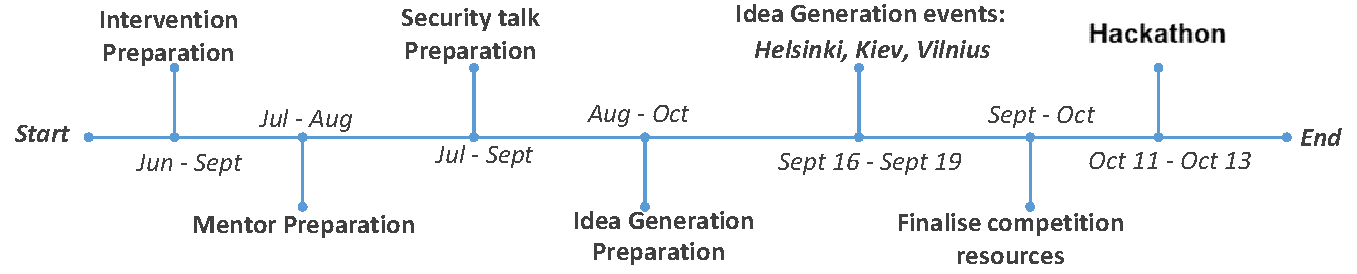
\includegraphics[width=\linewidth]{timelinehack.pdf}
  \caption{Timeline of the hackathon activities} \label{Fig:timeline} 
 % \vspace{-20pt}
\end{figure*}

\subsection{Data collection}
We selected three teams (denoted as A, B, and C) for data collection in this study. Data collected included observational data, questionnaires, and post-hackathon interviews. We will elaborate on how data collected from these data sources contribute to answering the research questions.

At the hackathon event, we moved between the teams to observe the participants. The observation method included monitoring at intervals and recording the responses of the participants to the interventions to influence learning in cybersecurity.
Reactions such as attentiveness to security talks, positive interactions with mentors reported when discussing with a sample of participants, and perceived satisfaction of participants to the project indicated reactions to respective interventions. We also recorded other aspects that may contribute to understanding the learning experience of the participants, such as teamwork, team process, or leadership influence.  
We did not observe the teams throughout the hackathon as we perceived the early, mid and late phases of the hackathon to be necessary.
We use the recorded observations to evaluate if the participants able to achieve learning gains with the introduced interventions as well as other team aspects (\hr{RQ1}). 

After the hackathon event, we conducted a post-hackathon questionnaire. This questionnaire covered the participants' perception of learning gains from the interventions and learning benefits from completing the security project. It also records the participants' perception of specific team properties such as size, team familiarity, leadership, skill diversity, and collaboration process.
Sample questions include; 
\begin{enumerate}
    \item To what extent was your decision to participate in the cybersecurity hackathon motivated by:[\textit{options list}]
    \item How did you work together on your project during the hackathon? [\textit{options list}]
    \item To what extend do you agree with the following statements about your cybersecurity learning experience at the hackathon? [\textit{[options list]: Talking with my mentors helped me learn more about cybersecurity}]
    \item Please indicate your level of agreement with the following statements related to the satisfaction with your learning experience: [\textit{options list}]
\end{enumerate}

From the selected teams, we chose 2 participants per team for an interview to discuss the hackathon experience, learning gains at the hackathon, and the hackathon outcome (i.e., security project worked on). 
These participants were selected because they either held a vital role in the team (i.e., team lead) or by observation, seemed to contribute significantly to the team.
%and analyzed for participants to provide a better comprehension of perceived individual and team learning experiences. (\hr{RQ2})
The interviews lasted from 25 to 30 minutes.
A sample of questions asked during the interviews include;
\begin{enumerate}
    \item How was the hackathon from your perspective in the form of: What did you do after you arrived? How did you see the event play out? 
    \item Did you attend the pre-event? What idea did you develop? How else did you prepare for this hackathon?
    \item What were the outcomes as a result of learning? [mentors, security talks, team members, working on the project]
    \item How do you perceive the outcome of the hackathon? Were you satisfied? How did you see your teamwork? 
    \item What security issues did your project address? What security considerations did you place on the [process of creation of the product, the outcome of the project].
    \item Did you discover anything new as regards security during the hackathon? How did you discover this?
    \item What about the continuity of your project? Have you use anything learned during the hackathon already? Are you planning to use it in the future? 
    \item Do you still use any security knowledge gained during the hackathon?
\end{enumerate}
The data from the post-hackathon interviews enabled us to evaluate how well the interventions worked for the team participants in encouraging perceived cybersecurity learning. 
We are also able to suggest improvements to interventions, from the post-hackathon interview responses (\hr{RQ2}).

\subsection{Analysis procedure}\label{Sec:analysisprocedure}
First, we discuss the journeys each selected team and the impacts of the introduced interventions on the teams. This analysis provides us with background information on the teams' activities during the hackathon and team properties (size, team familiarity, skill diversity, leadership).

We then compared cybersecurity learning for the teams alongside bloom's taxonomy learning dimensions.
Bloom's taxonomy describes levels of learning where each category of Remember, Understand, Apply, Analyze, Evaluate, and Create form the learning dimensions \cite{bloom1956taxonomy,krathwohl2009taxonomy}.
Bloom's taxonomy is uses data from team observations to assess which team was able to achieve maximum learning gains with the introduced interventions. We can analyse the processes by which the participants encountered and worked with knowledge provided through the interventions by comparing the teams journeys.

%We focused on the team as our unit of analysis, analysing how the participants in a team responded to the interventions of idea generation, security talks at the event, mentor feedback process and the competition design type. Some interesting parts of the hackathon i.e., satisfaction with the final product, team demographics i.e (size, skill diversity, familiarity, leadership) were included where they may have affected the learning experience.
%Data concerning the team demographics, i.e., skill diversity was derived by calculating the similarity of perceived team skills and then revert the result by subtracting it from one.
%We use data from different questionnaire questions to assess the different interventions (see Table \ref{tab:teambinter}). This qualitative data will complement further analysis done using the observation and interview. For this mapping, we followed a strategy \cite{braun2006using} by creating and applying initial codes to the interviews based on our research questions and interesting points that could also help answer research questions. We compared the findings for each team to assess the perceived learning of one team over another.

Lastly, we evaluate how well the interventions worked for the team participants in encouraging perceived cybersecurity learning using data from the questionnaires and interviews. This also reveals the shortcomings of the introduced interventions in fostering learning, where we suggest improvements to the interventions.

\section{Findings}
This section outlines the journeys of each selected team, the perception of each learning intervention on each team, and the differences between teams in relation to their learning process with the introduced interventions. All aspects we discuss are reflected in Table \ref{tab:teambinter}.
\begin{table}[h]
    \caption{Calculated means and standard deviations used in qualitative data analysis}
    \label{tab:teambinter}
    %\centering
    \begin{tabular}{|p{0.22\linewidth}|p{0.42\linewidth}|p{0.1\linewidth}|p{0.1\linewidth}|p{0.1\linewidth}|}\hline
	Intervention & Significant \newline questionnaire Question (see Appendix) &  Team A & Team B & Team C \\ \hline
	Idea generation & Q3, Q13 & $\emptyset$ & 2.25 & 2.5  \\ \hline
	Security Talks  & Q13 &  4 & 3 & 3.67   \\ \hline
	Mentor Feedback  & Q13 &  3.5 & 3 & 3.33 \\ \hline
	Competition style \newline (Final Product) & Q4, Q13, Q14, Q15 & 3.3 & 3.3 & 2.7   \\ \hline
	\multirow{8}{*}{**Team properties} & size (Q5) & 6 & 6 & 5  \\\cline{2-5}
	%& skills (Q1**, Q3) & 0.5 , 1 & 0.5,2.5 & $\emptyset$, 1  \\ \hline
	& team familiarity (Q9) & 1.125 & 4 & 1  \\ \cline{2-5}
	%& motivation (Q2) & 3 & 3.92 & 2.56  \\ \cline{2-5}
	%& preparation (Q4) & 1.25 & 2.75 & 1.33  \\ \cline{2-5}
	& leadership (Q7) & yes & yes & yes  \\ \cline{2-5}
	& skill diversity (Q8) & 0.6 & 0.7 & 0.4  \\ \cline{2-5}
	& collaboration process (Q10,Q11) & 3.81 & 4.56 & 4.125  \\ \cline{2-5}
	& satisfaction(Q12, Q13) & 3.9 & 2.85 & 3.35  \\ \hline
    \end{tabular}
    %*Partial evaluation as Q3 did not apply \\
    *Not interventions, but team properties that were found interesting in analysis.
\end{table}


\subsection{Team A}
The leader of team A (A01) proposed the idea for the project in the idea generation session at the main hackathon event. A01 derived the idea from ``\textit{a security problem from studies''} (A01) of the hackathon and intended to create a tool for enterprises to visualize security aspects. A01 formed a diverse (\textit{0.6}) 6-member team, and they did not know each other before the hackathon ($m = 1.125$).  \textit{``Ideation continued during the hackathon because the idea was not properly prepared''} (A01), and completed after discussions in the team and mentor feedback. The idea was refined to ``\textit{be targeted at company risk management team to help visualise and communicate security risk scenarios to upper management}''(A01).

At the security talk sessions, team A members reported cybersecurity learning gains from the talks ($m = 4$) and showed an understanding of the security domain while moving forward with the project. A01 highlighted on the ``\textit{educating experience about risk management and what is missing in the cybersecurity field}'' (A01) presented at the security talks.

In the creation of the final product, A01 highlighted that there was ``\textit{support by experienced team members to complete tasks}'' for the project. The team leader (A01) fostered learning within the team \textit{``holding everything together, monitoring and identifying the needs of each team members for completing tasks''}. A01 described how teamwork grew and how ``\textit{everybody was eager to work and contribute in any way they could}''; ``\textit{some team members had no prior experience to security, but they tried to learn and contribute}'' (A01). A01 thus reported that the team members ``\textit{went definitely beyond their current skills}''. The team leader (A01) was involved in  \textit{``monitoring and identifying the needs of each team members for completing tasks''}, and mentors supported these responsibilities were necessary to adjust scoping of the project. A01 presented updates to the mentors about the project progress, getting feedback from mentors about moving forward to the prototype stage. Talking and interacting with mentors was reported to help the team learn more about cybersecurity ($m = 3.5$).

At the end of the hackathon event, team A presented the security prototype to judges for evaluation. Although team A did not win a prize at the competition, the team members reported, a moderate learning experience from building the final product ($m = 3.3$) and an agreement on the satisfaction level from the event ($m = 3.9$), with individual comments about the \textit{``great event setup and mentoring''} (A01) and how \textit{``nicely organized''} (A02) the event was. However, A01 expressed that there will be no continuation in the project because it was \textit{``not quite sure, the market value for this type of project''} (A01).%, having less intent to continue with the project as opposed to another team member A02.


\subsection{Team B}
The leader of team B (B01) presented an idea developed at the pre-hackathon event. B01 highlights that attending the ideation event provided \textit{``a lot of support to [my] idea''}. The idea developed was to \textit{``make data security more desirable for startups and give them a badge''} (B01), thereby tackling the security awareness in startups issue. B01 presented the idea during the idea pitching session of the hackathon event and a little feedback provided by mentors. After ideation, B01 reports that team formation was easy. This is because B01 \textit{``was familiar with most of the team because [we] studied together at the university''}($m = 4$). B01 formed a diverse (\textit{0.7}) 6-member team.

At the security talk sessions, B02 explained that the security talks at the hackathon event were instrumental as the team \textit{``tried to gather all sorts of information on how to secure systems and gained knowledge''}. Team B members reported security gains from the talks ($m = 3$). Team B participants report learning experiences from the mentor feedback ($m = 3$) as it provided \textit{``an opportunity for [us] to explain our work progress''} (B02). B02 reported that \textit{``different mentors visited multiple times''}, and that the mentors  \textit{``visited to guide completing tasks''} (B02), but B01 reported that the multiple visits ``\textit{disrupted the flow of tasks}"(B01). B01 reports that mentors specifically provided feedback on the scoping of the project, and refinement of project content. % to define the life-cycle of different startups and the security implementations needed for each stage of the life-cycle as well as the business aspects.

In the creation of the final product, the team perceived their collaboration process to be efficient ($m = 4.56$). B01 mentioned that a \textit{``blackboard equipment for documenting the team's process and ideas, allowing [us] to see the big picture''}, thereby aiding collaboration between members of the team and between the team and mentors. 
The competition style of the hackathon, team B participants, reported learning experience($m = 3.3$) from accomplishing the task of building security content for the prototype.

Towards the end of the hackathon event, Team B pitched their project and presented the prototype for evaluation. Team B won a prize for a unique product developed and its perceived usefulness to the security community. Interestingly, there was a moderate satisfaction with the outcome of the project ($m = 2.9$). B01 raised an issue with a team member leaving the team unexpectedly halfway through the hackathon with the resources already gathered by the team. Continuation of the project following the competition style intervention was encouraged by the incentive prize awarded to the team project. Although B01 reported that the team intends to continue with the project, we learned from both B01 and B02 that the provided incentive might not be useful to its continuation.


\subsection{Team C}
The team lead (C01) pitched an idea during the idea generation session of the hackathon event. Although C01 attended the ideation pre-hackathon event, the idea pitched at the main hackathon event was not prepared during the pre-hackathon event. C01 pitched the idea to \textit{``create a binary betting platform for smart contracts''} on a blockchain platform. However, mentors provided feedback that the presented idea did not readily give a solution to current security issues and asked C01 to think more of the security solution. C01 formed a less diverse ($\textit{0.4}$) 5-member team, constituting mainly of developers interested in developing a blockchain-based solution.

Once team formation was complete, the participants in team C continued idea refinement with the mentor feedback. C02 stated that the initial idea \textit{``didn't seem like a good idea for a security hackathon, so [we] needed to connect it to a security topic''}. Thus, a new idea was formed based on blockchain, where the team decided on \textit{``an availability insurance smart contract for service providers''} (C02). The team leader (C01) provided progress reports on development to the mentors, who contributed as much feedback as possible on enhancing the proposed security prototype. The participants of team C report learning experience from the provided mentor feedback ($m = 3.33$). Although were no individual reports from the participants of team C about learning experiences from the security talk sessions, questionnaires responses from team C participants report learning gains from the security talk intervention ($m = 3.67$).

The participants in team C report learning experience ($m = 3.3$) by researching the security aspects of the prototype. The team perceived their collaboration process to be efficient ($m = 4.25$). C02 highlighted that this was due to the team's high interest in development using blockchain. Towards the end of the event, Team C pitched the final prototype for evaluation. After evaluation, Team C did not win a prize at the event and reported moderate satisfaction with the outcome of the project ($m = 2.85$). C02 mentioned that the moderate outcome might be due to the difficulty faced in ideation. There were no intentions of the participants to continue with the project idea.


\subsection{Team Comparison} \label{teamcomparison}
In this section, we compare the learning levels between the team's A, B and C based on the knowledge of the team's activity, and other observations at the hackathon (see section \ref{Sec:interventions}). According to our findings, team B showed the most learning gains followed by team B then team C. These comparisons are summarised in Table \ref{tab:bloomteamcomp}. In the following, we discuss how the teams were observed to use the different interventions in order to achieve learning gains.


Team A was able to show the ability to recognise relevant security knowledge to provide specific security information gained through the security talks. The participants (A01, A02) were able to recall the security risk management concepts discussed in the security talks, and discussed about these concepts in relation to their security solution. 
Team B has also shown the ability to remember security knowledge from the security talks intervention. B01 presented the security idea of a platform that encourages data security, related to security issues raised in the security talks. Team C participants talked about the availability security aspects of blockchain, recalling knowledge from security talk sessions. Teams A, B, and C attained the \textbf{Remember} process category.

Teams A and B showed the ability not only to remember and recall but interpret and explain the security concepts gained through the interventions. Team A also showed an understanding of security issues during and security talks leading to the generation of a security relevant idea and discussions of the understand security issues and its impact in a security risk-aware business environment, and team B for the start-up environment.  Thus the teams A and B attained the \textbf{Understand} process category.

Teams A and B were able to apply the security knowledge gained during the ideation sessions, following mentor feedback and in the process of building a unique security solution.
Team A (A01) was able to incorporate feedback from mentors to focus on resources to visualise and communicate security risk scenarios. Team B (B01) was able to apply mentor feedback in defining the security aspects within the life-cycle of target start-ups. Team B also showed the application of security knowledge gained by research on the security aspects within start-up life cycles. Team C participants, in interviews, did not readily show the application of gained security knowledge in its process and blockchain based product. Thus, the teams A and B attained the \textbf{Apply} process.

Teams A, B, and C were given the chance to present their developed security solutions. However, only team B was able to show how the security knowledge gained through interventions relate to the overall purpose and structure of the given solution. Team B respondents presented an analysis of how the introduction of each intervention affected each task, sub-task or process in the development of the final prototype. The team B achieved the \textbf{Analyse} process. 

\begin{table}[h]
    \caption{Team Learning Comparison}
    \label{tab:bloomteamcomp}
    \centering
    \begin{tabular}{|p{0.15\linewidth}|p{0.14\linewidth}|p{0.14\linewidth}|p{0.12\linewidth}|p{0.12\linewidth}|p{0.13\linewidth}|p{0.14\linewidth}|}
    \hline
      %& \multicolumn{6}{c|}{The cognitive process dimension}  \\ \hline
	 & Remember knowledge & Understand knowledge & Apply knowledge & Analyse knowledge & Evaluate knowledge & Create knowledge\\ \hline
%Factual Knowledge &   List & Summarize & Classify &   Order & Rank & Combine \\ \hline
	%Conceptual &   Describe &   Interpret &   Experiment & Explain & Assess & Plan \\ %\hline
%	Procedural & Tabulate & Predict & Calculate & Differentiate & Conclude & Compose \\ \hline
	Team \newline Knowledge & A, B, C & A, B & A, B & B & -- & -- \\ \hline
%	Meta-cognitive &  Appropriate use &   Execute & Construct & Achieve & Action &   Actualise \\ \hline
    \end{tabular}
\end{table}


\section{Discussion}
%\textit{Look into previous literature about the subject and compare with what we have now.}
In this section, we evaluate how the teams A, B, and C perceived the usefulness of the interventions in cybersecurity learning and suggest improvements to the interventions to answer \hr{RQ2}.


\subsection{Evaluation of Interventions} \label{evalintervention}
An analysis of the teams in relation to the interventions allows us determine how well (or not) each intervention worked for the teams.

Team B seems to have benefited from the \textbf{idea generation} intervention was instrumental in creating the security solution, and as a result, winning the competition. Of all three teams, team B was able to take the most advantage of this intervention, and having more time to work on the idea, resulting in a more mature security idea to be worked on during the event. Team B reports that this was possible because the team lead (B01) attended the ideation sessions at the pre-hackathon event and began developing the security idea already.
Although C01 attended the ideation sessions at the pre-hackathon event, C01 did not develop an idea at the event. Also, none of the participants of team A attended the pre-hackathon event.
As such, these teams had fewer chances in involving in as much cybersecurity learning from idea generation as team B.
%Team A and C did not take full advantage of this intervention leading to much time put into idea generation at the event.

Teams A and B appeared to have benefited most from \textbf{security talks} while team C showed little to no benefit. This could be because the security talks provided held high relevance to teams A and B's security solutions. 
A01 reported that the security talk on security risk management was relevant to their security risk visualisation solution. B01 reported that the security talk on start-up security awareness provided the required cybersecurity knowledge relevant to their security solution.
C01 reported that the security talks were not particularly relevant to their blockchain solution but were only useful to provide general security knowledge. It thus appears important that talks need to be tailored towards team needs in order to be perceived as useful.

Team B seems to have benefited most from the \textbf{mentor feedback} intervention in achieving cybersecurity learning as opposed to other teams. This could be because of the high amount of interaction with diverse mentors. B02 reported that different mentors visited the team at multiple times to provide an expert perspective on work progress, although B01 reported that mentoring became disrupted due to multiple visits.
Teams A and C, however, did not report high interaction with diverse mentors as with team B. 
A01 reported mentor interaction in ideation and in supporting the completion of set tasks for the security solution, while C01 only report mentor interaction in ideation. Thus, reducing the teams' chances of involving in as much cybersecurity learning as team B. 
It appears crucial that mentoring needs to be organised appropriately to ensure an adequate amount of mentor interaction.

In the \textbf{competition style} intervention, Team B appears to have benefited the most. B01 reported that the intervention encouraged rapid knowledge gathering and application of the security knowledge to product creation.
This could be as a result of culminating factors including idea generation, team formation, and team properties such as team familiarity, collaboration, satisfaction and leadership, all within the competition constraints. 
A01 reported not achieving this learning outcome because too much time was spent on ideation, causing a race with time to complete the security solution adequately. C02 also reported difficulties faced in ideation as an issue in achieving the learning outcomes of this intervention.


\subsection{Suggestions for Improvement}
We suggest suggestions to improve the introduced interventions based on our analysis in Section \ref{evalintervention}. This answers \hr{RQ2}.

%\subsubsection{Idea generation.}
%With proper idea generation, team A was able to produce more mature ideas, focus on building the security product and involving in more cybersecurity learning. 
Based on our findings we would suggest to design \textbf{idea generation} in a way that emphasizes the need for idea generation especially before the main hackathon event.
%\subsubsection{Security talks.}
For \textbf{security talks}, based on our findings, three suggestions can be proposed for future iterations.
First, the content of the security talks can be more domain-generic. Another option is to appropriately scope the ideas generated at the hackathon to the context of the hackathon. Finally, we develop the security talks only after idea generation is completed, so that the talks are more domain-specific and have maximum effect of offering adequate security knowledge to participants.
%\subsubsection{Mentor feedback.}
Based on our findings, we suggest that the \textbf{mentor feedback} intervention be handled with excellent coordination not to disrupt the team process. 
We suggest that a designated member of the team (most likely the team leader) with knowledge of the team's process, stand in between the mentors and the team when necessary, to handle explanations of the teams progress, and what the team needs in mentoring to prevent multiple disruptions.
%\subsubsection{Competition style.}
%In the \textbf{competition style} we suggest 
%However, B01 reported that the incentive provided was not relevant to the needs of the specific product because the product was content-specific, and thus, building the content and adapting it to the needs of real-life stakeholders was a priority over marketing. B01 stated that they ``\textit{expected to have interviews and discussions with stakeholders and startups to build proper security content, but the program did not provide this}". A suggestion is to understand the future needs of a project and provide an incentive that accommodates these needs.

\subsection{Limitations}
The aim of our study was to develop and evaluate specific interventions that can foster cybersecurity learning during a hackathon. While it appeared reasonable to conduct an action research study \cite{lewin1946action} there are certain limitations associated with this particular study design. We developed specific interventions and studied three teams that participated in a hackathon over a limited period of time that had specific backgrounds and goals for attending the hackathon. Despite selecting teams thoroughly it is not possible to generalize findings beyond our study context since studying a different setting with different teams, during a different hackathon working on different projects might yield different results. Moreover the researchers conducting the study were involved in the planning of the hackathon which can affect the reported findings despite our best efforts to refrain from interfering during the hackathon itself. We also abstained from making causal claims instead providing a rich description of the observed behavior and reported perceptions of teams based on which we discuss differences in how they reacted to the different proposed interventions.

\section{Conclusion}
This research explores the security hackathon designs, analysis of methods to influence learning in a security hackathon, analysis of the hackathon process and evaluation of perceived learning as a result of the introduced interventions.

\bibliographystyle{splncs04}
\bibliography{references}

\end{document}
